\section{Przegląd istniejących rozwiązań}

%------------------------------------------------

\begin{frame}
\frametitle{Robot Velma}
\begin{figure}
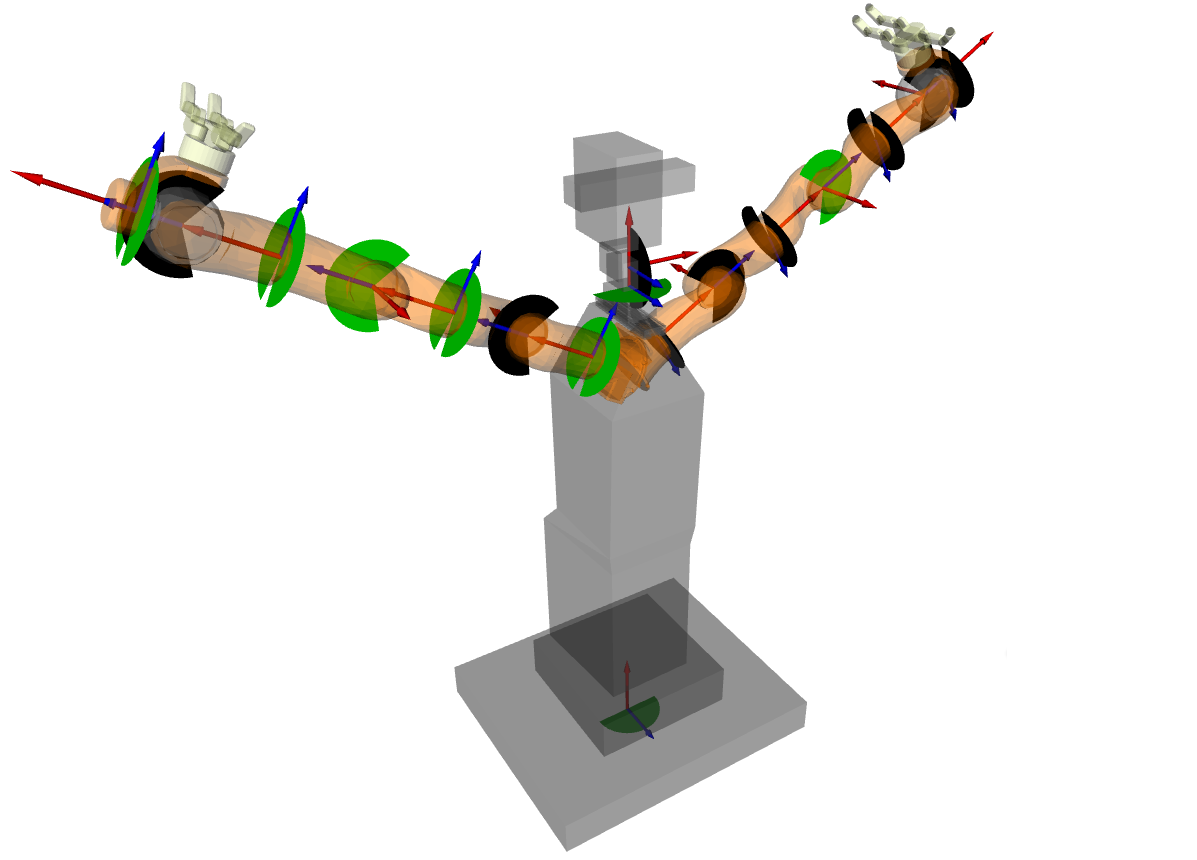
\includegraphics[scale=0.21]{./images/velma_joints.png}
\setcaptioncitation{\texttt{rcprg-ros-pkg.github.io/velma\_docs/}  \cite{docsVelma}}
\caption{\normalsize{Wizualizacja robota Velma z zaznaczonymi stopniami swobody}}
\end{figure}
\end{frame}

%------------------------------------------------

\begin{frame}
\frametitle{Robot Velma}
\begin{figure}
	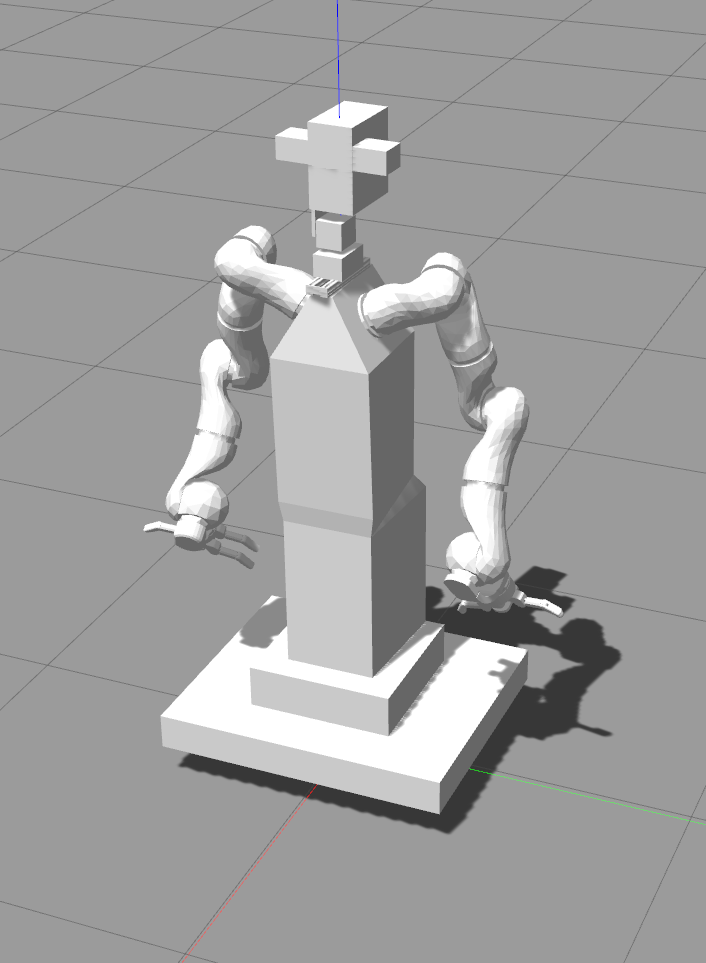
\includegraphics[scale=0.20]{./images/velma_gz_cropped.png}
	\caption{Robot Velma w symulatorze Gazebo}
\end{figure}
\end{frame}

%------------------------------------------------

\begin{frame}
\frametitle{Robot Velma}
Robot Velma składa się z \cite{docsVelma}:  
\begin{itemize}
	\item obrotowego korpusu
	\item dwóch manipulatorów KUKA LWR
	\item dwóch chwytaków BarrettHand
	\item szyi o dwóch stopniach swobody
	\item kamery Kinect XBOX 360
	\item czujników sił i momentu
	\item sztucznej skóry
\end{itemize}
\end{frame}

%------------------------------------------------

\begin{frame}
\frametitle{Struktura symulatora}
\begin{block}{Zasada działania}
	Symulator korzysta z komponentów OROCOS działającym w czasie rzeczywistym, wykorzystujących Gazebo
	do uzyskania informacji o otoczeniu.
\end{block}
\end{frame}

%------------------------------------------------

\begin{frame}
	\frametitle{Struktura symulatora}
	\begin{figure}
	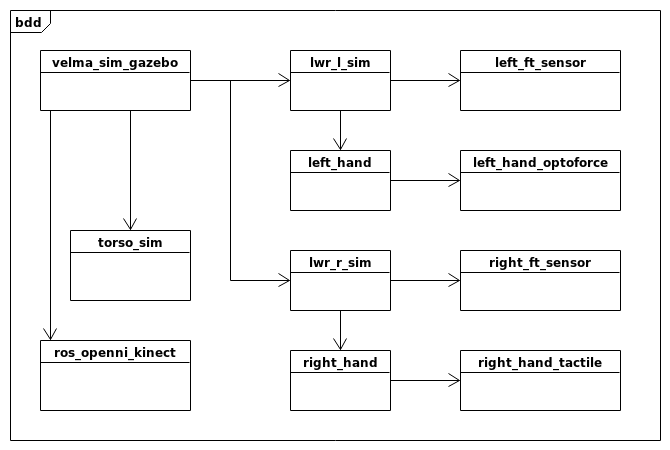
\includegraphics[scale=0.40]{./images/velma_sim_bdd.png}
	\caption{Struktura symulatora części manipulacyjnej z kamerą}
	\end{figure}
\end{frame}

%------------------------------------------------

\begin{frame} 
\frametitle{Robot Velmobil}
\begin{figure}
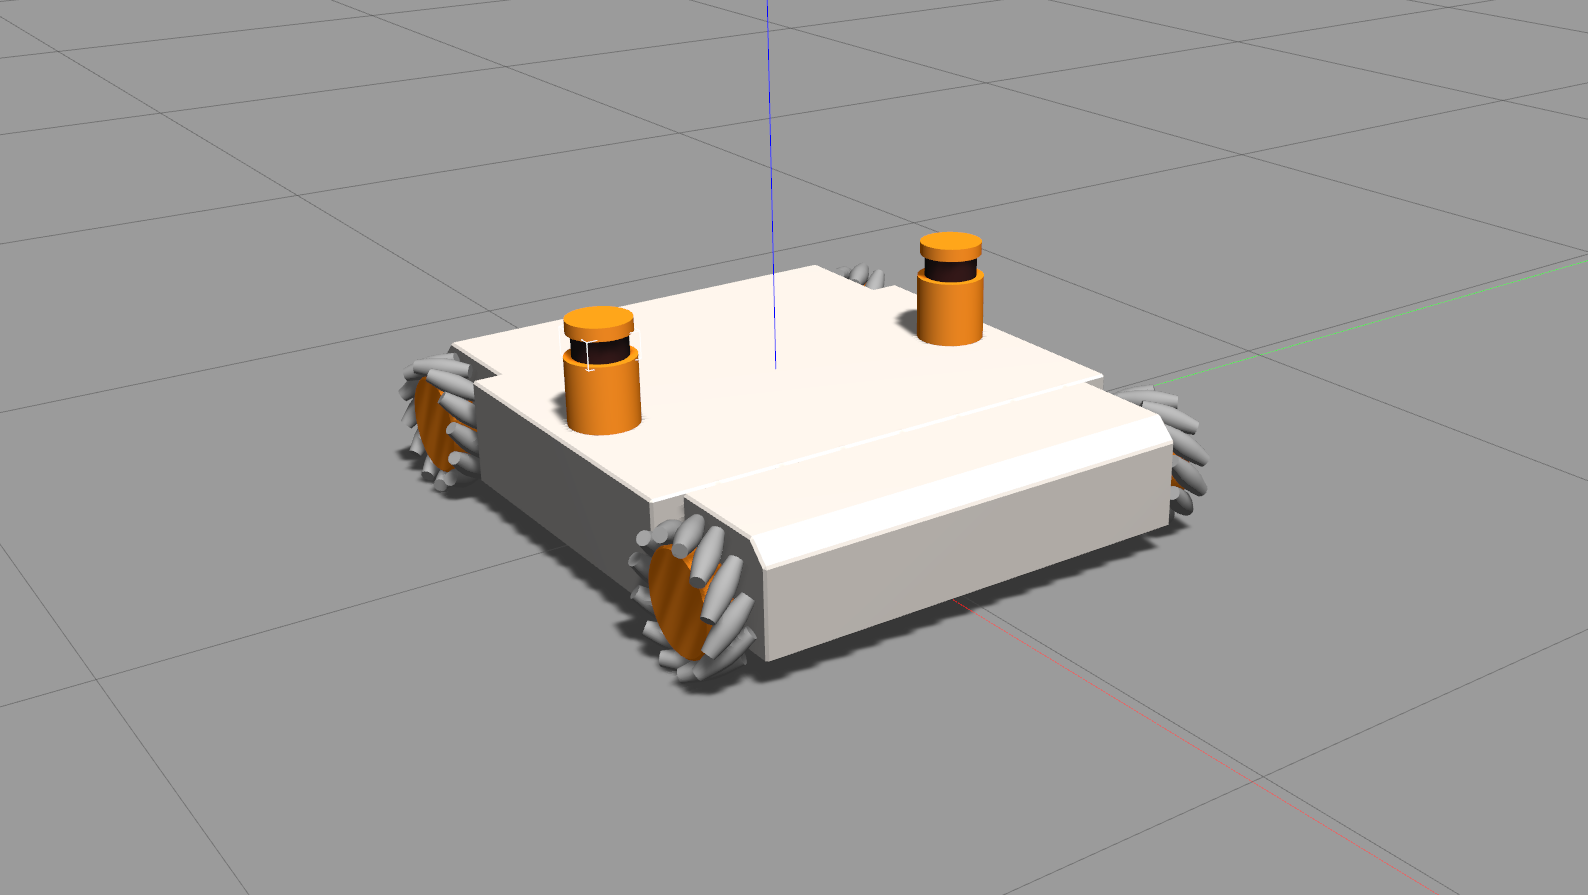
\includegraphics[scale=0.20]{./images/omnivelma_gz.png}
\caption{Baza mobilna robota w symulatorze Gazebo}
\end{figure}
\end{frame}

%------------------------------------------------

\begin{frame}
\frametitle{Robot Velmobil}
Robot Velmobil posiada \cite{walas}:  
\begin{itemize}
	\item 4 koła szwedzkie
	\item dwa skanery laserowe LIDAR
	\item jednostkę inercyjną
	\item enkodery % jakie enkodery
\end{itemize}
\end{frame}

%------------------------------------------------

\begin{frame}
\frametitle{Struktura symulatora}
\begin{block}{Zasada działania}
Symulator bazy mobilnej został przygotowany w postaci wtyczki do Gazebo. 
Jest on znacznie prostszy niż symulator korpusu i nie jest przystosowany
do pracy z rzeczywistym sprzętem.
\end{block}
\bigskip
Sterowanie pojazdem
odbywa się poprzez odbieranie i nadawanie wiadomości na tematach.
\begin{itemize}
	\item \texttt{/omnivelma/vels} - ustawienie prędkości kół
	\item \texttt{/omnivelma/encoders} - kąt i prędkość kół z enkoderów
\end{itemize}
\end{frame}
